\subsection{Fourier-Zernike Basis}

We defined Fourier series for periodic functions and Zernike Polynomials for functions defined on a disc. Now, consider a stellarator or a tokamak. We can express any function inside those geometries by Fourier series in the toroidal direction ($\zeta$) and by Zernike Polynomials in a toroidal cross-section ($\zeta = $ constant).

\begin{equation}
    f(\rho,\theta,\zeta) = \sum_{l}^{}\sum_{m}^{}\sum_{n}^{} c_{lmn} \mathcal{Z}_l^m (\rho,\theta) \mathcal{F}^n(\zeta) \label{fourier-zernike-coef}
\end{equation}
With the previous definitions from \ref{fourier-basis-cos}, \ref{fourier-basis-sin} and \ref{zernike-poly}, we can write a function depending on $\rho, \theta$ and $\zeta$ as,
\begin{align}
    f(\rho,\theta,\zeta) =  \mathlarger{\mathlarger{\sum}}_{n=0}^{N}c_{lmn} &cos(n\zeta)\mathlarger{\mathlarger{\sum}}_{l=0}^{L}\begin{cases}
        \mathlarger{\sum}_{|m|=0}^{l} \begin{cases}
            \mathcal{R}_l^{m}(\rho) cos(m\theta) & \text{for } m\geq0 \\[.2cm]
            \mathcal{R}_l^{|m|}(\rho) sin(|m|\theta) & \text{for } m<0
        \end{cases}& \text{for } l \text{ even} \\[.7cm]
        \mathlarger{\sum}_{|m|=1}^{l} \begin{cases}
            \mathcal{R}_l^{m}(\rho) cos(m\theta) & \text{for } m\geq0   \\[.2cm]
            \mathcal{R}_l^{|m|}(\rho) sin(|m|\theta) & \text{for } m<0
        \end{cases}& \text{for } l \text{ odd}
        \end{cases} \\[0.7cm]
        +& \mathlarger{\mathlarger{\sum}}_{n=1}^{N}c_{lmn} sin(n\zeta)\mathlarger{\mathlarger{\sum}}_{l=0}^{L}\begin{cases}
        \mathlarger{\sum}_{|m|=0}^{l} \begin{cases}
            \mathcal{R}_l^{m}(\rho) cos(m\theta) & \text{for } m\geq0 \\[.2cm]
            \mathcal{R}_l^{|m|}(\rho) sin(|m|\theta) & \text{for } m<0
        \end{cases}& \text{for } l \text{ even} \\[.7cm]
        \mathlarger{\sum}_{|m|=1}^{l} \begin{cases}
            \mathcal{R}_l^{m}(\rho) cos(m\theta) & \text{for } m\geq0   \\[.2cm]
            \mathcal{R}_l^{|m|}(\rho) sin(|m|\theta) & \text{for } m<0
        \end{cases}& \text{for } l \text{ odd}
        \end{cases}
\end{align}

This starts to get a bit messy. Let's represent possible modes ($l, m$ and $n$ combinations) in terms of an array where each row is a mode. For example, take $l$, we can call it radial resolution from now on, $L$ = 3, and take $n$, we can call it the toroidal resolution, $N$ = 3. Corresponding basis function for each mode $l, m$ and $n$ can be written as,
\begin{align}
    \mathcal{Z}_l^m (\rho,\theta) \mathcal{F}^n(\zeta) = \begin{cases}
        \mathcal{R}_l^{m}(\rho) cos(m\theta) cos(n\zeta)  \hspace{1cm}& \text{for } m\geq0 \text{ and } n\geq0\\[.1cm]
        \mathcal{R}_l^{m}(\rho) cos(m\theta) sin(n\zeta)  \hspace{1cm}& \text{for } m\geq0 \text{ and } n<0\\[.1cm]
        \mathcal{R}_l^{|m|}(\rho) sin(|m|\theta) cos(n\zeta)  \hspace{1cm}& \text{for } m<0 \text{ and } n\geq0\\[.1cm]
        \mathcal{R}_l^{|m|}(\rho) sin(|m|\theta) sin(n\zeta)  \hspace{1cm}& \text{for } m<0 \text{ and } n<0\\[.1cm]
    \end{cases}   \label{fourier-zernike-basis}
\end{align}

\begin{figure}[H]
    \centering
    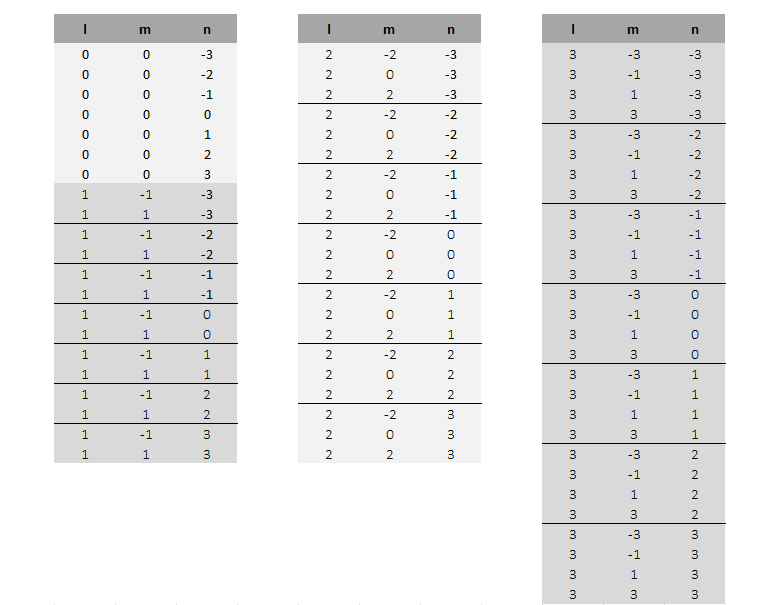
\includegraphics[width=0.8\textwidth]{lmn-table.png}
\end{figure}

In addition to basis functions and modes given in the table, there are also coefficients for each mode, let's call them $c_{lmn}$. So, in total, for $L = N$ = 3 case (where $L$ and $M$ are defined as in theory not DESC version), there are 70 modes. In general, the number of modes can be expressed in terms of chosen resolutions as,

\begin{equation}
    \begin{split}
        \textit{Total Number of Modes} \hspace{0.5cm} &= \hspace{0.5cm} \mathlarger{\mathlarger{\sum}}_{n=-N}^{N} \hspace{0.2cm} \mathlarger{\mathlarger{\sum}}_{l=0}^{L} \hspace{0.2cm} (l+1) \\[0.3cm]
        &= \hspace{0.5cm} (2N+1) \left(\frac{L(L+1)}{2}+L+1\right)\\[0.3cm]
        &= \hspace{0.5cm} \frac{1}{2} (2N+1) (L+1)(L+2)
    \end{split}
\end{equation}


